\mychapter{Teori}


\section{Kryptering}


\section{Blockchiffer}


\subsection{Körlägen}


\subsubsection{ECB}
\acrfull{ecb} är en av det enklaste blockchiffer körlägena som finns.
\acrshort{ecb} i sig är ganska lätt att förstå och bygger i huvudsak bara på
att man delar upp den data man vill kryptera i delar kallade block och tar sedan varje
block för sig och kör genom algoritmen, vilket tydligt visas i
Figur \ref{fig:ecb-mode-enc} \& \ref{fig:ecb-mode-dec}.
\footfullcite{modesofoperation}

Figur \ref{fig:ecb-mode-enc} visar hur \acrshort{ecb} fungerar vid kryptering.
Här visas hur varje block för sig krypteras med hjälp av en blockchiffer algoritm
tillsammans med den givna nyckeln.

\begin{figure}[H]
    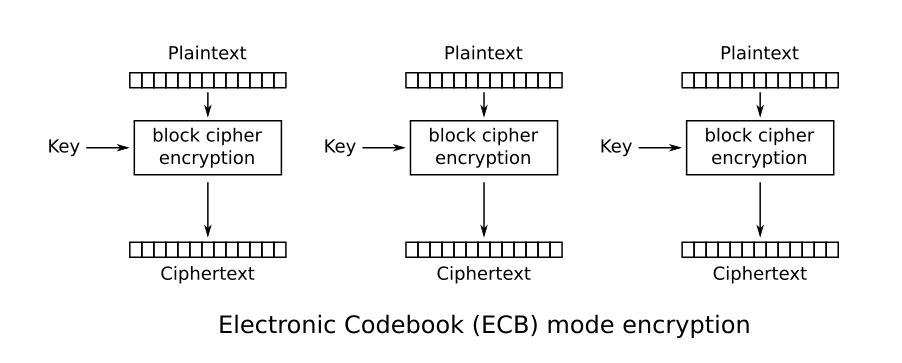
\includegraphics[width=\textwidth]{ECB_encryption.png}
    \captionsource{\acrlong{ecb} kryptering}{{\cite{ecb-mode-enc-ref}}}
    \label{fig:ecb-mode-enc}
\end{figure}

Figur \ref{fig:ecb-mode-dec} visar istället hur \acrshort{ecb} fungerar vid
dekryptering, vilken är en till stort sett identisk operation med det enda undantaget
att blockchiffret körs i dekrypterings läge istället för krypterings läge.

\begin{figure}[H]
    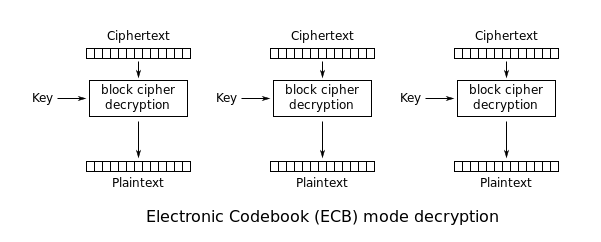
\includegraphics[width=\textwidth]{ECB_decryption.png}
    \captionsource{\acrlong{ecb} dekryptering}{{\cite{ecb-mode-dec-ref}}}
    \label{fig:ecb-mode-dec}
\end{figure}

På grund av \acrshort{ecb} körlägets simplicitet så finns det dock även ett ganska
stort problem med detta körläge. Det handlar om att \acrshort{ecb} inte på något
sätt förhindrar att två block med samma innehåll som krypteras inte resulterar i
ett identiskt krypterat block.\footcite{modesofoperation}

Vad detta innebär är att för större mängder data
är att det börjar bildas mönster i skiffertexten. Detta är något som väldigt
tydligt visar sig ifall man krypterar en bild, vilket går att se när man jämför
figur \ref{fig:pi-original} \& \ref{fig:pi-ecb}.
Det här faktumet är även varför \acrshort{ecb} inte är ett säkert körläge
och därför inte används näst intill aldrig i praktiken.\footcite{modesofoperation}

\subsubsection{CBC}
\acrlong{cbc} är ett av de mest vanligen använda körlägena för många blockchiffer.

\footcite{modesofoperation}

\begin{figure}[H]
    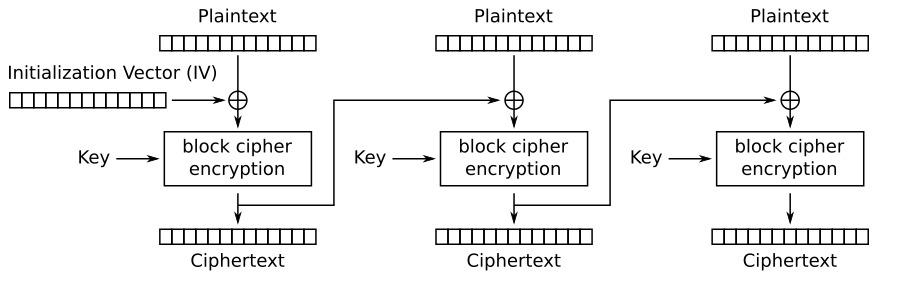
\includegraphics[width=\textwidth]{CBC_encryption.png}
    \captionsource{\acrlong{cbc} kryptering}{{\cite{cbc-mode-enc-ref}}}
    \label{fig:cbc-mode-enc}
\end{figure}

\begin{figure}[H]
    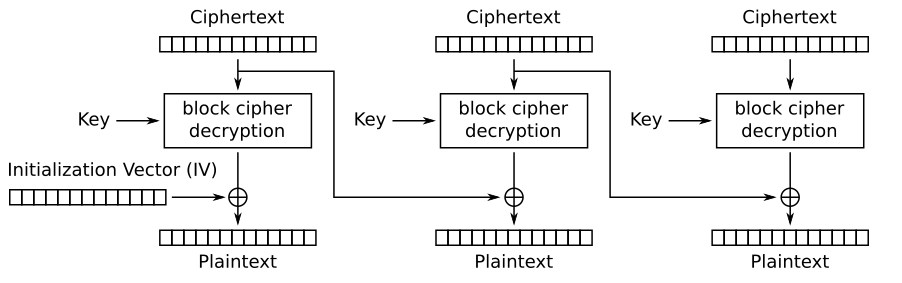
\includegraphics[width=\textwidth]{CBC_decryption.png}
    \captionsource{\acrlong{cbc} dekryptering}{{\cite{cbc-mode-dec-ref}}}
    \label{fig:cbc-mode-dec}
\end{figure}

\subsubsection{OFB}


\section{Symetrisk \& Asymmetrisk Kryptering}
Symetrisk och asymetrisk kryptering handlar om hur nycklar används i olika
krypteringsalgoritmer. För symetriska krypterings algoritmer så betyder detta
att samma nyckel är vad som används för både kryptering och dekryptering.

\footfullcite{symencrypt}

\section{AES}


\subsection{Finite Fields}


\subsection{AES S-Box}


\subsection{Struktur}


\subsubsection{SubBytes operation}
SubBytes operationen bygger på ...

\subsubsection{ShiftRows operation}


\subsubsection{MixColumns operation}


\subsubsection{AddRoundKey operation}


\subsection{Nyckel utökning}


\subsubsection{RotWord}


\subsubsection{SubWord}


\subsubsection{Rcon}


\subsection{AES-128bit}


\subsection{AES-192bit}


\subsection{AES-256bit}

